\documentclass[a4paper, 12pt]{article}%тип документа

%%%Библиотеки
	%\usepackage[warn]{mathtext}	
	\usepackage[T2A]{fontenc} % кодировка
	\usepackage[utf8]{inputenc} % кодировка исходного текста
	\usepackage[english,russian]{babel} % локализация и переносы
	\usepackage{caption}
	\usepackage{listings}
	\usepackage{amsmath,amsfonts,amssymb,amsthm,mathtools}
	\usepackage{wasysym}
	\usepackage{graphicx}%Вставка картинок правильная
	\usepackage{float}%"Плавающие" картинки
	\usepackage{wrapfig}%Обтекание фигур (таблиц, картинок и прочего)
	\usepackage{fancyhdr} %загрузим пакет
	\usepackage{lscape}
	\usepackage{xcolor}
	\usepackage[normalem]{ulem}
	\usepackage{hyperref}

%%%Конец библиотек




%%%Настройка ссылок
	\hypersetup
	{
		colorlinks=true,
		linkcolor=blue,
		filecolor=magenta,
		urlcolor=blue
	}
%%%Конец настройки ссылок


%%%Настройка колонтитулы
	\pagestyle{fancy}
	\fancyhead{}
	\fancyhead[L]{Лабораторная работа}
	\fancyhead[R]{Талашкевич Даниил, группа Б01-009}
	\fancyfoot[C]{\thepage}
%%%конец настройки колонтитулы



							\begin{document}
						%%%%Начало документа%%%%


%%%Начало титульника
\begin{titlepage}

	\newpage
	\begin{center}
		\normalsize Московский физико-технический институт \\(госудраственный 			университет)
	\end{center}

	\vspace{6em}

	\begin{center}
		\Large Лабораторная работа по электричеству\\
	\end{center}

	\vspace{1em}

	\begin{center}
		\large \textbf{Измерение магнитного поля Земли [3.1.3]}
	\end{center}

	\vspace{2em}

	\begin{center}
		\large Талашкевич Даниил Александрович\\
		Группа Б01-009
	\end{center}

	\vspace{\fill}

	\begin{center}
	Долгопрудный \\2021
	\end{center}
	
\end{titlepage}
%%%Конец Титульника



%%%Настройка оглавления и нумерации страниц
	\thispagestyle{empty}
	\newpage
	\tableofcontents
	\newpage
	\setcounter{page}{1}
%%%Настройка оглавления и нумерации страниц


					%%%%%%Начало работы с текстом%%%%%%
					
\textbf{Цель работы:} измерение зависимости сопротивления полупроводниковых образцов различной формы от индукции магнитного поля. \\

\textbf{Используемое оборудование:} электромагнит, милливеберметр или миллитесламетр (на основе датчика Холла), вольтметр, амперметр, миллиамперметр, реостат, образцы монокристаллического антимонида индия (InSb) $n$-типа.
                    
\section{Теоретическое введение}

В работе исследуется эффект зависимости электрического сопротивления от магнитного поля на примере диска Корбино (см. рис.).

\begin{figure}[h]
    \centering
    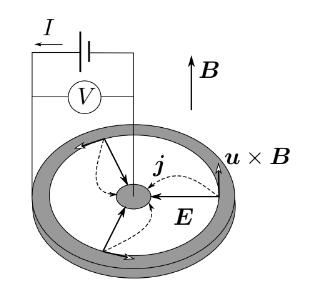
\includegraphics[width = 5 cm]{images/1.png}
    \caption{Диск Корбино}
    \label{karb}
\end{figure}

При отстутствии магнитного поля, направленного перпендикулярно плоскости диска, по диску течёт ток, определяемый по закону 

\begin{equation}
    I = \frac{U}{R_0}, \; R_0 = \frac{\ln{\frac{r_2}{r_1}}}{\sigma_0 2 \pi r h}
\end{equation}

Однако при включении магнитного поля индукции $B$ на частицы-переносчики тока начинает действовать сила Лоренца, из-за чего траектория частиц увеличивается в расстоянии, проходимом между двумя точками с фиксированной разницей потенциалов $U$.

В этом случае проводимость  равна 

\begin{equation}
    \sigma_r = \frac{\sigma_0}{1 + (\mu B)^2}
\end{equation}

Закон Ома преобразовывается в следующий вид:

\begin{equation}
    I = \frac{U}{R}, \; R = R_0 (1 + (\mu B)^2)
\end{equation}

Таким образом, зависимость $I(U)$ поменялась из-за геометрических особенностей диска Корбино. Такой эффект называют геометрическим магнетосопротивлением. В этой работе будут исследоваться зависимость сопротивления диска от магнитного поля, проверяться выше записанные формулы и исследоваться как влияет характер зависимости геометрических форм на зависимость $R(B)$.

\section{Экспериментальная установка}

Для исследование зависимости $R(B)$ используется следующая методика:

\begin{enumerate}
    \item Используется калибровка электромагнита (источника магнитного поля): находится зависимость индукции создаваемого магнитного поля от тока в контуре электродвигателя $B(I_m)$ (или $I_m(B)$), который регистрируется амперметром $A_1$, чтобы в дальнейшем считать величину магнитного поля с помощью тока в контуре $I_m$.
    \item При постоянной силе тока $I_0$, которая настривается с помощью сопротивления реостата в контуре с источником питания, меняется величина индукции магнитного поля, тем самым меняется напряжение $U$, подаваемое на диск Корбино. Исследуется зависимость $R(B)$ через калибровочную кривую и зависимость $U(I_m)$.
    \item Проводится тот же самый опыт с прямоугольной пластинкой с исследованием зависимости её сопротивления $R(B)$.
\end{enumerate}

\begin{figure}[h!]
    \centering
    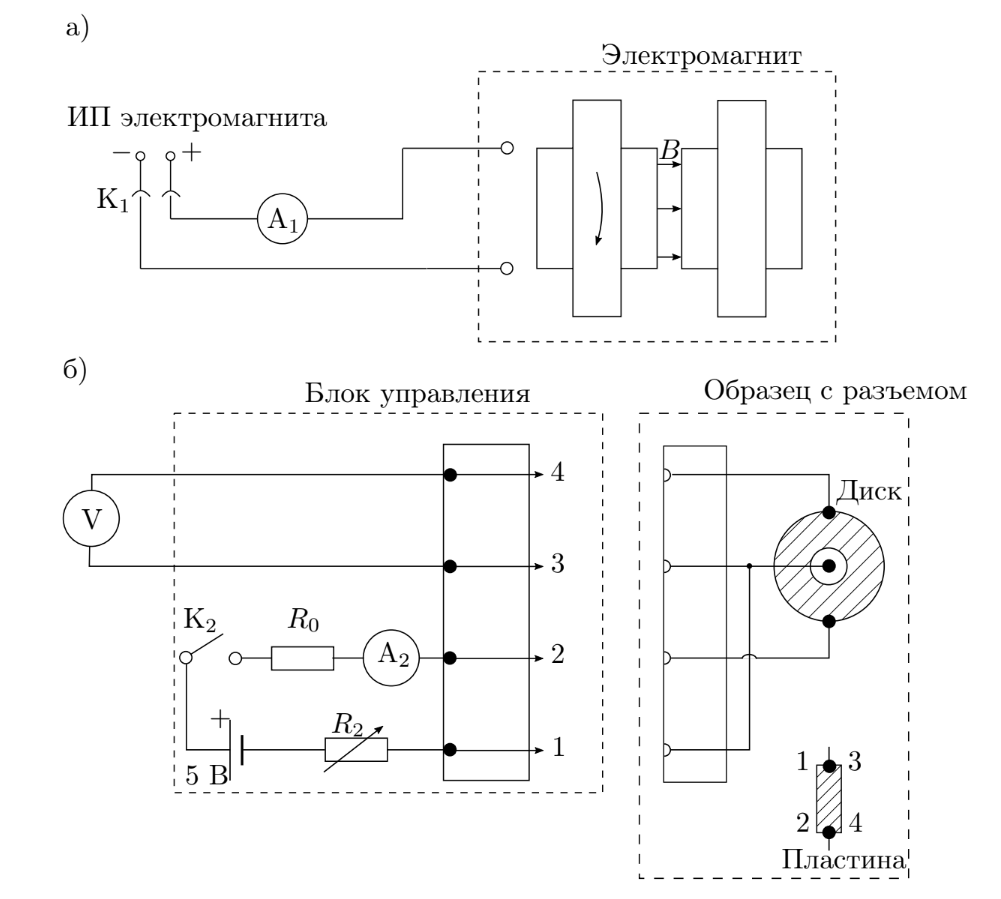
\includegraphics[width = 13 cm]{images/2.png}
    \caption{Схемы экспериментальных установок}
    \label{scheme}
\end{figure}


\section{Ход работы}

\subsection{Подготовка приборов к работе}

Включим вольтметр кнопкой "Сеть"

Присоединим диск Корбино через разъём к цепи питания. Убедившись, что реостат $R_{2}$ выведен на минимум тока, включим в сеть блок управления и тумблером $\mathrm{K}$ подключим образец.

Теперь определим диапазон изменения силы тока через образец. Для этого снова уберем ток до нуля и временно отключим образец от цепи. 

Установим все ручки регулировки источника питания магнита (GPR-11H30D) на минимум сигнала и включим источник в сеть. Установим обе ручки регулировки тока на максимум.

Используя ручки регулировки напряжения $R_{1}$ (сначала $fine$, затем $coarse$), определим диапазон изменения силы тока через электромагнит, чтобы выбрать, каким шагом следует увеличивать ток при калибровке магнита. 

Получили следующий диапазон изменения силы тока через электромагнит $0.05 - 0.40$ А.


\subsection{Калибровка электромагнита}

Сперва ознакомимся с устройством и принципом работы измерителя магнитной индукции Ш1-10.

Теперь при помощью прибора Ш1-10 исследуем зависимость индукции $B$ магнитного поля в зазоре от тока $I_{M}$ через обмотки магнита.

Проведем измерения магнитной индукции для 8 значений тока $I_{\mathrm{M}}$ через электромагнит. Так же убидились, что в отсутствие тока через магнит индукция $B$ практически равна нулю.


\begin{table}
\begin{center}
\begin{tabular}{|c|c|}
\hline I, A & B , мТс	\\
\hline $0,05$ & $71,4$ 	\\
\hline $0,10$ & $125,7$ 	\\
\hline $0,15$ & $188,1$ 	\\
\hline $0,20$ & $247$ 	\\
\hline $0,25$ & $301$ 	\\
\hline $0,30$ & $338$ 	\\
\hline $0,35$ & $356$ 	\\
\hline $0,39$ & $371$ 	\\
\hline
\end{tabular}
\caption{градуировка $B$($I$)}
\end{center}
\end{table}

График полученной зависимости (и её аппроксимация):

\begin{center}
\begin{figure}[h]
    \centering
    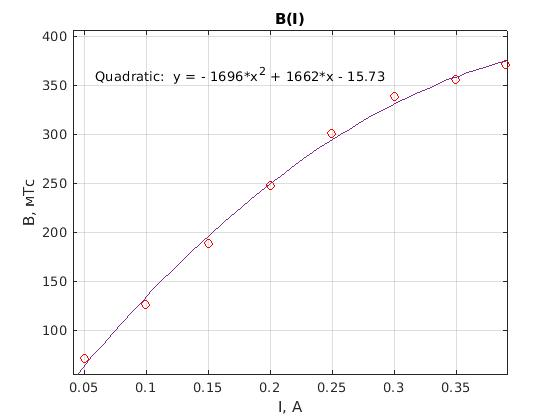
\includegraphics[width = 10 cm]{B(I).jpg}
    \caption{Измерение магнитных моментов шариков}
    \label{msh1}
\end{figure}
\end{center}

Видно, что при небольних значениях тока зависимость почти линейная, однако при больших видны значительные отклонения от прямой (парабола).


\subsection{Исследование магнетосопротивления образцов}

Подключим диск Корбино к электрической цепи. При помощи реостата $R_{2}$ установим ток через образец $I_{0} \simeq 25$ мА. Измерьм падение напряжения на образце в отсутствие магнитного поля. XX

Вставим держатель с диском в зазор электромагнита. Снимим зависимость напряжения $U$ на образце от тока $I_{M}$ через обмотки магнита при фиксированном токе через образец $(I_{0} \simeq 25$ мА $) .$


Перевернув образец, убедимся, что результат измерения не зависит от направления магнитного поля. XX


Теперь  вместо диска Корбино подключим к измерительной цепи образец, имеющий форму пластинки. Реостатом $R_{2}$ установим в образце ток 10 мА. Измерим падение напряжения на образце в отсутствие магнитного поля.


Снимим зависимость напряжения $U$ на образце от тока через магнит при постоянном токе $I=10$ мА через образец. При измерениях длинная сторона образца должна быть направлена поперёк поля, а средняя (ширина) в одной серии опытов располагается вдоль, а в другой - поперёк поля.

полученный данные: 

XX

Таблица с размерами диска и характеристик приборов.


\section{Обработка результатов}



\section{Вывод}



\section{Литература}

\begin{enumerate}
\item \textbf{Лабораторный практикум по общей физике:} Учебное пособие. В трех томах. Т. 2. Электричество и магнетизм /Гладун А.Д., Александров Д.А., Берулёва Н.С. и др.; Под ред. А.Д. Гладуна - М.: МФТИ, 2007. - 280 с.

\end{enumerate}		
		


\end{document}